\section{\heiti 引言}

随着信息技术飞速发展,“数字法院”建设已成为全球司法现代化的重要趋势。这使得对智能化司法审判解决方案的需求日益迫切,尤其是在刑事案件审判领域。该领域的核心目标是提升司法判决的准确性、一致性和效率~\cite{aletras2016predicting}。在此背景下,法律判决预测(LJP)作为法律人工智能领域的基础性、关键性研究任务,受到学术界和实务界的广泛关注。LJP通过分析案件事实描述,自动预测法院判决结果,辅助法官及其他法律从业者提升案件处理效率。

LJP技术的早期研究主要依赖人工构建的规则系统和传统统计机器学习方法\cite{katz2017general,keown1980mathematical},例如支持向量机(SVM)\cite{boella2011using,kim2015legal}。Sulea等人~\cite{sulea2017exploring}构建了一种结合多个SVM分类器输出平均概率的集成系统。该模型以案情事实描述和时间跨度信息为输入,能够输出判决结果、法律范围和估算判决日期等信息。Katz等人~\cite{katz2017general}使用随机森林,从案情描述中提取有效特征,预测美国最高法院的判决结果。然而,这些方法未能有效挖掘深层文本特征。由于其人工设计的特性,这些方法需要大量人力成本,难以广泛应用于其他领域。
\begin{figure*}[htbp]
	\centering
	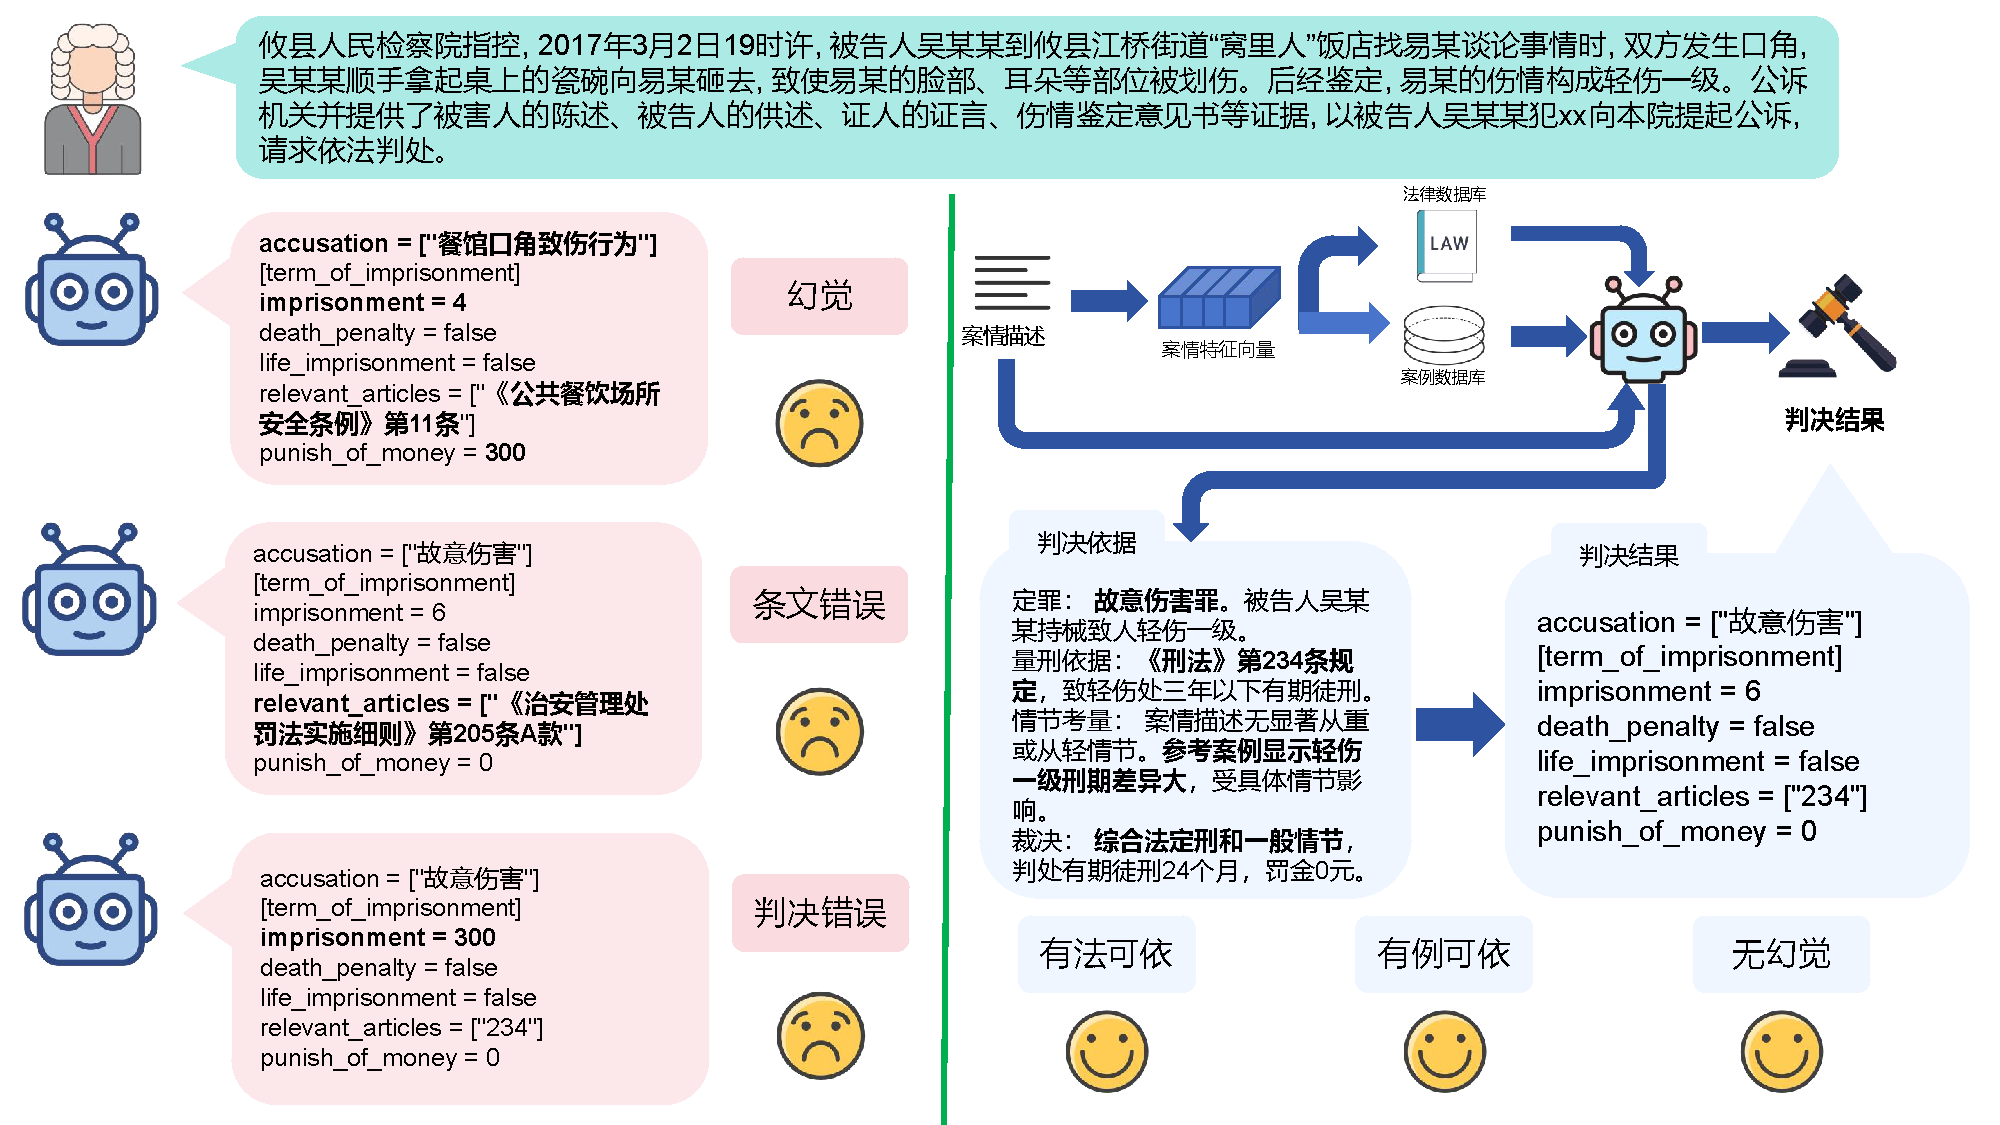
\includegraphics[width=1\textwidth]{fig/motivation.pdf}
	\caption{基于法条约束与类案融合的可解释司法判决预测动机}
	\label{fig:motivation}
\end{figure*}
此外,许多早期深度学习LJP模型如同“黑箱”般运作,其决策过程缺乏透明度和可解释性。模型的不可解释性构成了其在司法实践中推广应用的主要障碍\cite{ling2017program,ma2021law,nye2021show}。法官难以干预模型的审判逻辑或理解其预测依据,从而削弱了模型的实用价值。缺乏可解释性还可能引发伦理问题,尤其当模型从历史数据中学习到潜在偏见时,可能导致不公正或不一致的判决结果~\cite{luo2017learning,lv2022improving}。

尽管大型语言模型(LLM)因其卓越的语言理解能力而备受期待~\cite{jiang2023legal},但在法律领域的直接应用暴露出若干固有缺陷。一个核心问题是LLM倾向于产生“幻觉”(Hallucinations),即生成与客观事实或用户输入不符的内容~\cite{lewis2020retrieval,zheng2021when}。在法律语境下,这可能表现为援引虚假判例、引言或内部引证,从而导致判决不公,甚至判决错误。研究表明,在处理特定法律查询时,LLM的幻觉率可能高达69\%至88\%~\cite{Dahl_2024}。这种现象通常源于模型在缺乏可验证法律依据的情况下,尝试进行推理或生成信息~\cite{zhong2020iteratively,zhong2020jec-qa}。

针对传统方法在可解释性和处理复杂法律逻辑方面的不足,以及通用LLM在直接应用中面临的幻觉、法律知识基础缺乏和专业推理能力弱等问题,本研究提出了一种基于法条约束与类案融合的可解释司法判决预测方法。该方法通过提取判决核心要素(即犯罪核心要素与证据核心要素),旨在减少判决过程中的干扰因素,提供准确且核心的信息。
此外,本研究还引入相似案例,旨在为LLM提供司法实践层面的参考,使其理解法律条文在具体情境下的应用方式,并学习裁判经验。最后,LLM作为核心推理引擎,对这些多源异构信息进行综合分析和推理。它综合考量法律原则、司法解释及类案判例的指导作用,输出结构化的判决结果。本研究的方法无需对整个大型语言模型进行重新训练,它将复杂的LJP任务分解为多个子任务,使得整个推理过程更为透明和模块化。与一些端到端的“黑箱”模型相比,这种设计不仅有助于提升整体预测的鲁棒性,还为理解和调试模型行为提供了便利。
